%!TeX root=../main.tex
\فصل{آشنایی با میکروکنترلرهای \متن‌لاتین{ARM} و نرم‌‌افزار \متن‌لاتین{STM32CubeIDE}}
\قسمت{مقدمه}
\begin{figure}[!h]
	\centering
	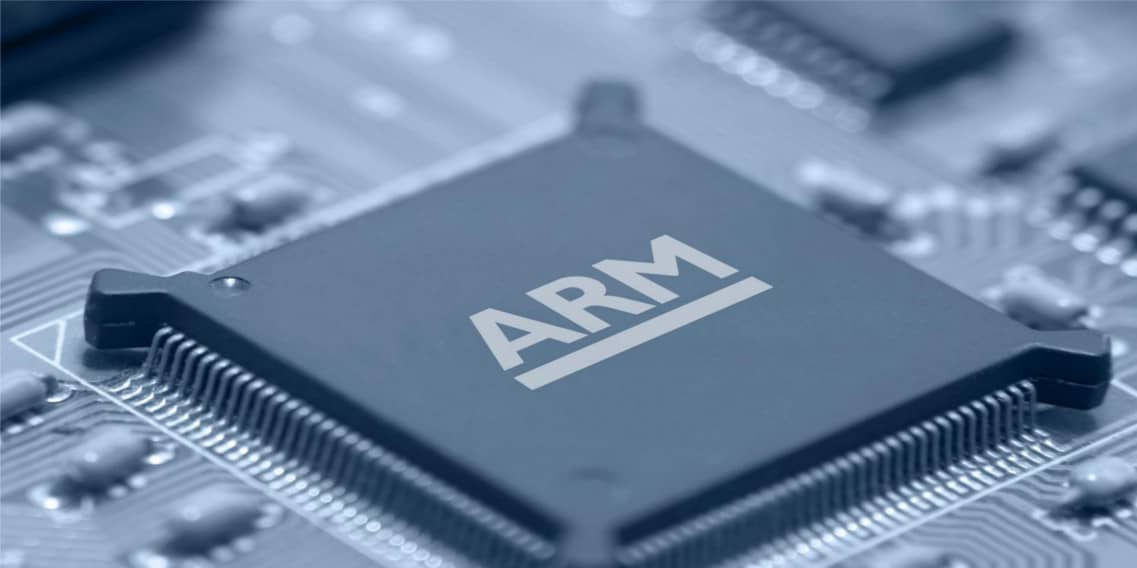
\includegraphics[width=0.7\linewidth]{Assets/arm.png}
\end{figure}

\متن‌لاتین{ARM} یک شرکت بریتانیایی و چندملیتی است که در زمینه نیمه‌‌رساناها و طراحی نرم‌افزارهای رایانه‌ای فعالیت می‌کند. نحوه تجارت این شرکت به این صورت است که گواهی‌نامه محصولات خود را به عنوان \متن‌لاتین{IP Core} به فروش می‌رساند و شرکت‌های دیگر از جملهNXP,  \متن‌لاتین{ST} \متن‌لاتین{Microelectronics}, \متن‌لاتین{Qualcomm}, \متن‌لاتین{Texas Xilinx}, \متن‌لاتین{Nvidia}, \متن‌لاتین{Atmel}, \متن‌لاتین{Apple} این لایسنس را خریداری کرده و محصولات خود را بر اساس آن تولید می‌کنند.

\قسمت{معماری \متن‌لاتین{ARM}}
معماری آرم\پانویس{ARM}، نوعی از معماری 32 بیتی و 64 بیتی، بر طبق طراحی \متن‌لاتین{RISC CPU} و ساختار پردازنده‌های رایانه‌ای است که به‌وسیله شرکت انگلیسی آرم هولدینگز\پانویس{Arm Holdings} طراحی شده‌است و به دلیل قیمت ارزان، سرعت بسیار زیاد، سخت‌‌افزارهای جانبی متعدد از جمله: \متن‌لاتین{CAN}, \متن‌لاتین{Ethernet}, \متن‌لاتین{UART}, \متن‌لاتین{SPI}, \متن‌لاتین{USB}, \متن‌لاتین{DAC}, \متن‌لاتین{ADC}, \متن‌لاتین{SDRam} و غیره، حافظه داخلی زیاد و توان مصرفی پایین (به ازای هر \متن‌لاتین{MHz}، جریانی از 0٫2 میلی‌آمپر تا 1 میلی آمپر مصرف می کنند). این پردازنده ها؛ اکثر سیستم های نهفته (مثل میکروکنترلرها، موبایل و تبلت و کلا سیستم هایی با حجم کوچک و امکانات بالا) از این پردازنده استفاده می کنند. معماری آرم از دهه ۱۹۸۰ میلادی تا به امروز در حال توسعه و گسترش است. \متن‌لاتین{ARM} مخفف \متن‌لاتین{Advanced RISC Machine} است و از آنجایی که این معماری براساس طراحی \متن‌لاتین{RISC} بنا شده‌‌است، برای هسته اصلی پردازشگر تنها به حدود ۳۵ هزار ترانزیستور نیاز است و این باعث می‌شود که پردازنده بسیار کم‌مصرف شود، کم‌تر داغ کند و نیازی به خنک‌کننده یا فن نداشته باشد بر خلاف معماری x86 به‌کار رفته در پردازنده‌های شرکت‌های اینتل و ای‌ام‌دی که نیازمند میلیون‌ها ترانزیستور هستند و همین مسئله باعث افزایش توان مصرفی و داغ شدن آنان می‌شود. شرکت آرم هولدینگز در سال ۲۰۱۴ معماری آرم با قابلیت پشتیبانی از دستورالعمل‌های ۶۴ بیتی در پردازنده‌های کورتکس-ای۵۳ و کورتکس-ای۵۷ توسط این شرکت تولید و عرضه شد.
از میان شرکت‌هایی که تولیدکننده میکروکنترلرهای 32بیتی هستند؛ میکروکترلرهای کمپانی \متن‌لاتین{ST} بیشترین محبوبیت را در صنعت دارد که قیمت پایین و در حین حال امکانات بالا و منابع اموزشی کامل از مزایای آن هستند.

\قسمت{میکروکنترلرهای شرکت ST}
\begin{figure}[!h]
	\centering
	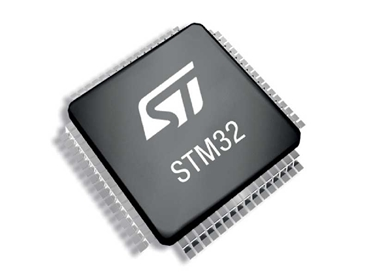
\includegraphics[width=0.7\linewidth]{Assets/stm.png}
\end{figure}
\زیرقسمت{مقدمه}
اس‌تی‌ام‌الکترونیکس، شرکت فرانسوی-ایتالیایی و چندملیتی تولیدکننده تجهیزات الکترونیکی و نیمه‌هادی‌ها می‌باشد، که دفتر مرکزی آن در شهر ژنو، سوئیس قرار دارد. این شرکت بر پایه میزان درآمد، به عنوان بزرگترین سازنده تراشههای نیم‌رساناها در اروپا محسوب می‌شود. در حالی که دفتر مرکزی شرکت اس‌تی‌میکروالکترونیکز و ستاد مدیریتی آن، در ژنو قرار گرفته‌است، ولی بخش عملیاتی این شرکت، در شهر آمستردام، هلند مستقر می‌باشد. دفتر مرکزی شعبه ایالات متحده این شرکت، در شهر کاپل، تگزاس قرار دارد. ستاد مرکزی شعبه آسیا اس‌تی‌میکروالکترونیکز در سنگاپور و ساختمان مرکزی شعبه ژاپن و کره جنوبی آن نیز، در توکیو مستقر می‌باشند. دفتر مرکزی شعبه چین این شرکت، در شهر شانگهای قرار گرفته‌است. شرکت اس‌تی‌مایکروالکترونیکس، در فهرست اولیه بازار بورس یورونکست ذکر شده‌است و به عنوان جزئی از شاخص فرانسوی کاک ۴۰ محسوب می‌شود. این شرکت همچنین در فهرست ثانویه از بازار بورس نیویورک و نیز بازار بورس ایتالیا، ذکر شده‌است.

\زیرقسمت{نحوه نام‌گذاری}
\begin{figure}[!h]
	\centering
	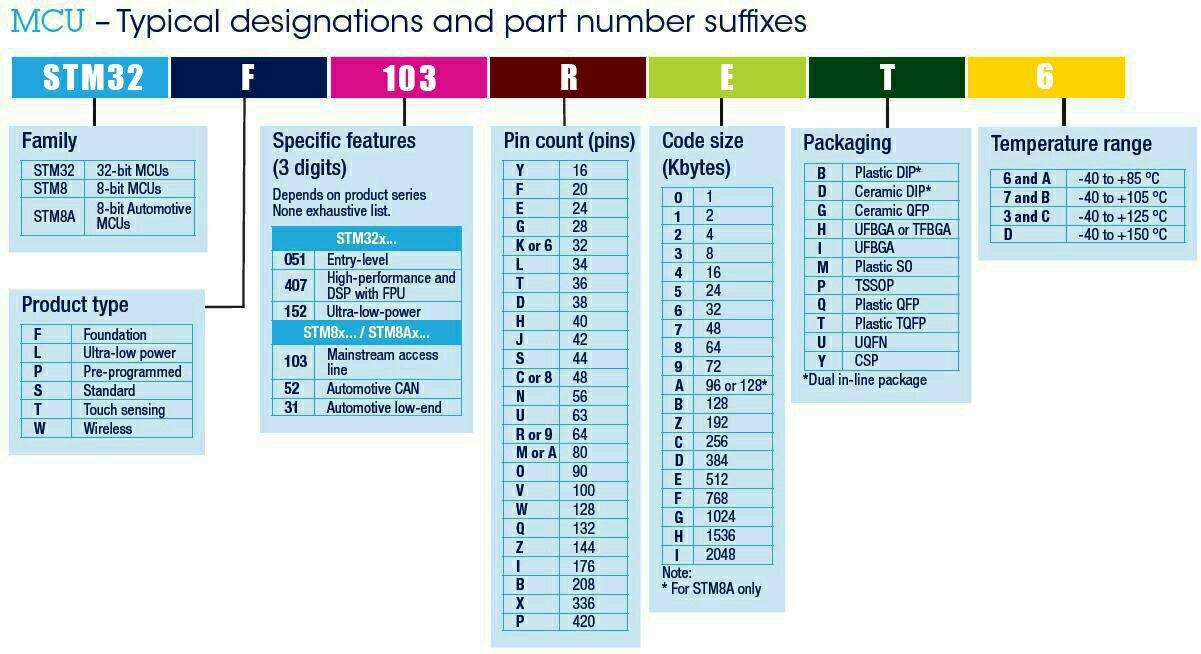
\includegraphics[width=\linewidth]{Assets/stmnaming.png}
	\caption{جدول نحوه نام‌گذاری میکروکنترلرهای شرکت \متن‌لاتین{ST}.}
	\label{fig:stmnaming}
\end{figure}

نام‌گذاری این میکروکنترلرها همواره با عبارت \متن‌لاتین{ST} شروع می‌شود که معرف شرکت سازنده خود می‌باشد. بعد از ترکیب \متن‌لاتین{ST} حرف \متن‌لاتین{M} می‌آید که نشانگر این است که محصول حاضر یک میکروکنترلر می‌باشد. بعد از \متن‌لاتین{STM} یکی از عبارات $32$، $8$ یا $8A$ را خواهیم دید که به ترتیب معرف میکروهای ۳۲بیتی، ۸بیتی و ۸بیتی \متن‌لاتین{Automotive} می‌باشد. تا این مرحله خانواده کلی محصول مورد نظر معرفی گردید و سپس نوبت به تشریح ویژگی‌های میکروکنترلر می‌رشد. کاراکتر بعدی در نام‌گذاری فقط شامل یک حرف انگلیسی می‌باشد و یکی از حروف F ،L ،P ،S ،T یا W است. این حروف نوع محصول را مشخص می‌کنند. به طور مختصر باید گفت که حرف F مربوط به محصولات \متن‌لاتین{Foundation}، حرف L مربوط به \متن‌لاتین{Ultra-low power}، حرف P محصولات \متن‌لاتین{Pre-programmed}، حروف S مختص \متن‌لاتین{Standard}، عبارت T برای \متن‌لاتین{Touch sensing} و در نهایت W برای معرفی محصولات \متن‌لاتین{Wireless} به کار می‌روند. سپس شاهد یک عدد سه رقمی خواهیم بود. این عدد (مخصوصا رقم سوم) با حرف قبلی در ارتباط است.  این عدد ویژگی‌های خاص هر خانواده میکروکنترلر رو نشان می‌دهد، از جمله معماری، طبقه‌بندی، حداکثر فرکانس، حداکثر حافظه \متن‌لاتین{SRAM} و حداکثر حافظه \متن‌لاتین{Flash}. به عنوان مثال عدد 103 در میکروکنترلرهای \متن‌لاتین{STM32F103} نشانگر این می‌باشد که معماری این میکرو \متن‌لاتین{Cortex-M3} در طبقه‌بندی \متن‌لاتین{Mainstream} با حداکثر فرکانس 72 مگاهرتز، حداکثر حافظه فلش ۱۰۲۴ کیلوبایتی و حداکثر حافظه اِس-رم ۹۶ کیلوبایتی می‌باشد. لازم به ذکر است این اعداد منحصر بفرد می‌باشد و تقریبا الگوی مشخصی ندارد. در این عدد رقم سوم (رقم صدگان) از اهمیت بیشتری برخوردار هستش و اطلاعات اصلی را همین رقم بیان می‌کند. بعد از این عدد دوباره شاهد یک حرف انگلیسی خواهیم بود. این حرف تعداد پین‌های میکروکنترلر مورد نظر را مشخص می‌کند. بعد از آن، یک عدد یا حرف می‌بینیم که بیانگر مقدار حافظه \متن‌لاتین{Flash} میکروکنترلر می‌باشد. توجه داشته باشید که عدد ۳ رقمی قبل مقدار حداکثری حافظه \متن‌لاتین{Flash} خانواده را مشخص می‌کرد ولی عدد یا حرف حاضر دقیقا مقدار این حافظه را در این میکروکنترلر برای ما بازگو می‌کند. بعد از این قسمت دوباره شاهد یک حرف انگلیسی خواهیم بود که برای ما مشخص می‌کند میکروکنترلر مورد بحث از چه نوع پکیجی برخوردار است و در نهایت باز شاهد یک عدد یا حرف انگلیسی خواهیم بود که مشخص کننده رنج دمای کاری میکروکنترلر مربوطه می‌باشد. به این صورت که A یا ۶ محدوده ۴۰- تا ۸۰ درجه سانتی‌گراد، B یا ۷ محدوده ۴۰- تا ۱۰۵ درجه، C یا ۳ محدوده ۴۰- تا ۱۲۵ درجه و D محدوده ۴۰- تا ۱۵۰ درجه را مشخص می‌کند. مطالب بیان شده به صورت کلی در شکل \رجوع{fig:stmnaming} قابل مشاهده است.

\زیرقسمت{انواع کتابخانه‌های مورد استفاده در میکروکنترلرهای ST}
\زیرزیرقسمت{CMSIS}
یک لایه نرم‌افزاری برای سخت‌افزار پردازنده‌های کورتکس M هست که توسط بنیاد \متن‌لاتین{ARM}، تعریف‌شده و فارغ از شرکت سازنده میکروکنترلر است. به عبارتی \متن‌لاتین{CMSIS} ارائه‌شده برای شرکتی چون \متن‌لاتین{ST} مشابه همان CMSISای است که برای شرکت فیلیپس یا شرکت‌های دیگر ارائه شده. این یکسان بودن موجب می‌شود تا اصطلاحاً \متن‌لاتین{Portability} برنامه نوشته شده، بالا رود.
درواقع شما به کمک \متن‌لاتین{CMSIS} یک‌بار برای میکرویی کد می‎‌زنید و با کمترین تغییرات ممکن، می‌توانید آن را بر روی میکرویی از شرکتی دیگر انتقال دهید. این لایه بیشتر از آنکه حاوی توابعی برای انجام کارهای مختلف با پریفرال‎‌های میکرو باشد، دارای تعریف‌های1 مختلف از رجیسترهای میکروکنترلر است. درنتیجه شما باید بیشتر دست‌به‌کار شوید و خودتان برای راه‌اندازی و استفاده از امکانات میکروکنترلر کد بزنید.
اگر بخواهم به‌صورت نه‌چندان دقیقی حرف‌های بالا را خلاصه کنم، باید بگویم \متن‌لاتین{CMSIS} تنها یکسری اسم است که بر روی آدرس رجیسترهای میکرو گذاشته‌شده تا ما بتوانیم راحت‌تر با این رجیسترها کارکنیم.

\زیرزیرقسمت{کتابخانه‌های \متن‌لاتین{SPL} و \متن‌لاتین{HAL}}
ازلحاظ کلی \متن‌لاتین{SPL} و \متن‌لاتین{HAL} شبیه هم‌اند. هر دو دارای توابع زیادی برای کار با قسمت‌های مختلف میکروکنترلر دارند و برخلاف \متن‌لاتین{CMSIS} صرفاً حاوی تعریف رجیسترها نیستند. بلکه از تعاریف ارائه‌شده در \متن‌لاتین{CMSIS}، در این دو استفاده‌شده است. \متن‌لاتین{SPL} قدیمی‌تر از کتابخانه \متن‌لاتین{HAL} است و هر دو توسط شرکت \متن‌لاتین{ST} توسعه داده‌شده‌اند. اما ظاهراً شرکت \متن‌لاتین{ST} علاقه‌ای به پشتیبانی و ادامه کار بر روی \متن‌لاتین{SPL} ندارد و درنتیجه تمرکز خود را بر روی توسعه هرچه بیشتر و بهتر \متن‌لاتین{HAL} گذاشته است. شما هم ممکن است قبلاً با کتابخانه \متن‌لاتین{SPL} کارکرده باشید و آن را بیشتر از \متن‌لاتین{HAL} بپسندید. با این ‌وجود بهتر است از رویه شرکت پیروی کنیم و هر چه زودتر خود را به کار با توابع \متن‌لاتین{HAL} عادت دهیم. چراکه علاوه بر اینکه دیگر از کتابخانه \متن‌لاتین{SPL} پشتیبانی نمی‌شود، برای میکروهای سری \متن‌لاتین{M7} و \متن‌لاتین{H7} هم این کتابخانه وجود ندارد.
بعد از انتشار کتابخانه \متن‌لاتین{HAL} بسیاری از افراد از این گلایه داشتند که این کتابخانه پردازش را سنگین می‌کند و درون توابع خود به چیزهایی می‌پردازد که برایشان لزومی ندارد. به همین دلیل \متن‌لاتین{ST} تصمیم گرفت در کنار این کتابخانه، کتابخانه‌ای سبک‌تر به اسم \متن‌لاتین{LL}\پانویس{Low Layer} ارائه دهد که سطح پایین‌تر از \متن‌لاتین{HAL} باشد. این‌گونه دست افراد در برنامه‌نویسی بازتر است. هرچند که خودشان بایست نکات گفته‌شده در دیتاشیت و رفرنس‌منوال را رعایت کنند. در پروژه‌های ایجادشده توسط \متن‌لاتین{CubeMX} ما می‌توانیم صرفاً با اضافه کردن خطی برای اینکلود این کتابخانه، در کنار کتابخانه \متن‌لاتین{HAL} از توابع \متن‌لاتین{LL} در قسمت‌هایی که می‌خواهیم، استفاده کنیم. اگر می‌خواهید در لایه بالاتر کد بزنید و البته کد نوشته‌شده را راحت‌تر برای میکرو دیگری از شرکت \متن‌لاتین{ST} نیز استفاده کنید، بهتر است سراغ \متن‌لاتین{HAL} بروید. اما اگر سرعت از اهمیت بیشتری برایتان برخوردار است و از شلوغی توابع \متن‌لاتین{HAL} فراری هستید، بهتر است با \متن‌لاتین{LL} برنامه خود را توسعه دهید.

\زیرقسمت{نرم‌افزار \متن‌لاتین{STM32CubeIDE}}
اخیرا شرکت \متن‌لاتین{ST Microelectronics} به‌دلیل ارائه نر‌م‌افزار \متن‌لاتین{STM32CubeIDE} محبوبیت زیادی در میان دیگر شرکت‌ها پیدا کرده است. این نرم‌افزار کار با میکروکنترلرهای این شرکت را برای توسعه‌دهندگان بسیار ساده تر کرده است. این نرم افزار \متن‌لاتین{IDE} بسیار قدرتمندی برای میکروکنترلر‌های این شرکت است و به راحتی می‌توان امکاناتی که در پروژه به آن نیاز داریم را تنها با چند کلیک فعال کنیم. پس از انتخاب مورد نظر کد را به صورت خودکار بر اساس تنظیمات انجام شده تولید می‌کند. تصویری از محیط تنظیم امکانات این برنامه در شکل \رجوع{fig:stm32cubeide} قابل مشاهده است.

\begin{figure}[!h]
	\centering
	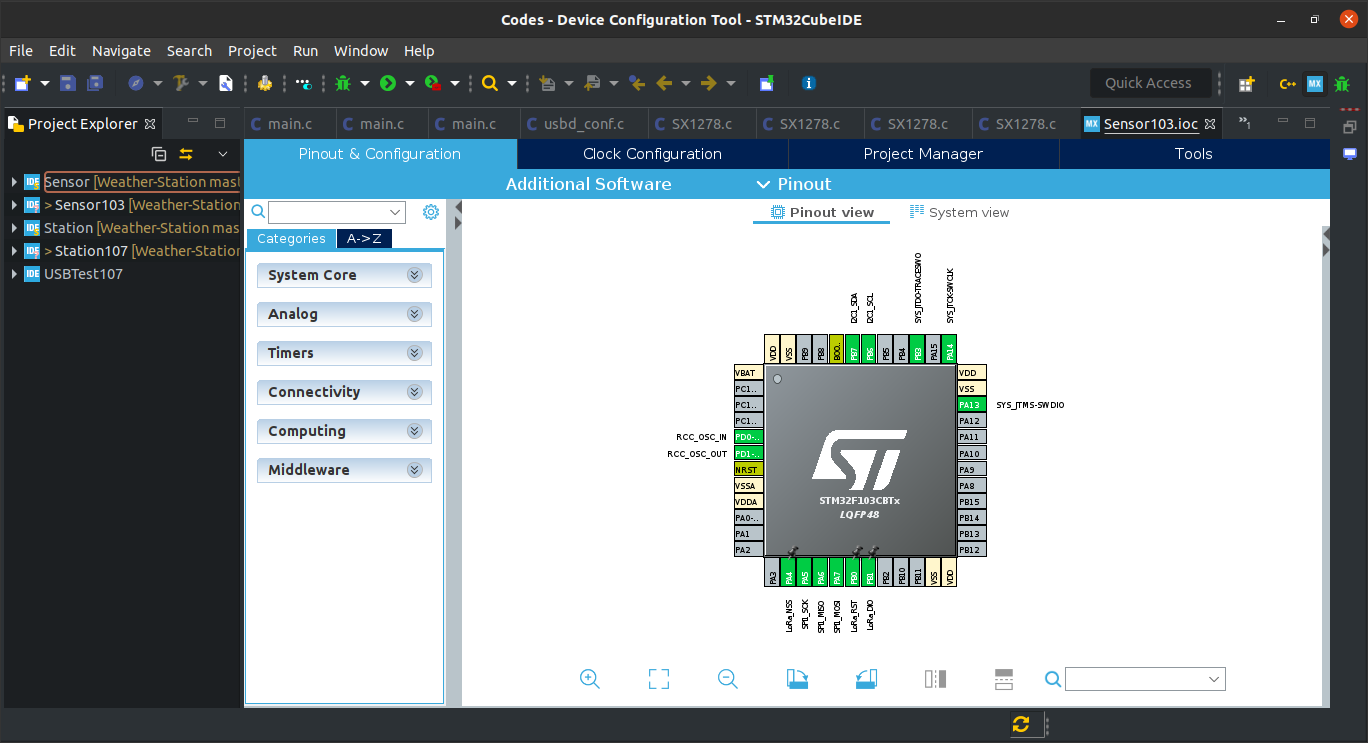
\includegraphics[width=\linewidth]{Assets/stm32cubeide.png}
	\caption{تصویر محیط نرم‌افزار \متن‌لاتین{STM32CubeIDE}.}
	\label{fig:stm32cubeide}
\end{figure}

نکته‌‌ای که در اینجا حائز  اهمیت است، این است تعدادی از خطوط برنامه توسط نرم‌افزار \متن‌لاتین{STM32CubeIDE} تولید شده است که نباید آن‌ها را حذف کنیم. دلیل وجود این کامنت‌ها این است که برنامه‌نویس کدهای خود را در قسمت‌های مشخص‌‌شده بنویسد و اگر پس از تکمیل پروژه نیاز به فعال کردن واحدی در میکروکنترولر داشت، بتواند دوباره به محیط تنظیمات وارد شد و پس از فعال‌کردن واحد موردنظر، تغییرات مورد نظر در کد اصلی بدون هیچ خطایی اعمال شود. در انتها نیز پس از اتمام کدنویسی، باید آن را توسط پروگرامر به میکروکنترلر انتقال دهیم. پروگرامر های مختلفی برای میکروکنترلرهای \متن‌لاتین{ARM} موجود است که پروگرمرهای \متن‌لاتین{JLINK} و \متن‌لاتین{STLINK} از  معروف‌ترین آن‌ها است که بسیاری از میکروکنترلرها را پشتیبانی می ‌کنند.
در شکل \رجوع{fig:programmers} تصاویری از پروگرامر‌های استفاده شده در پروژه را مشاهده می‌‌کنید.

\begin{figure}[H]
	\begin{subfigure}[b]{0.5\textwidth}
		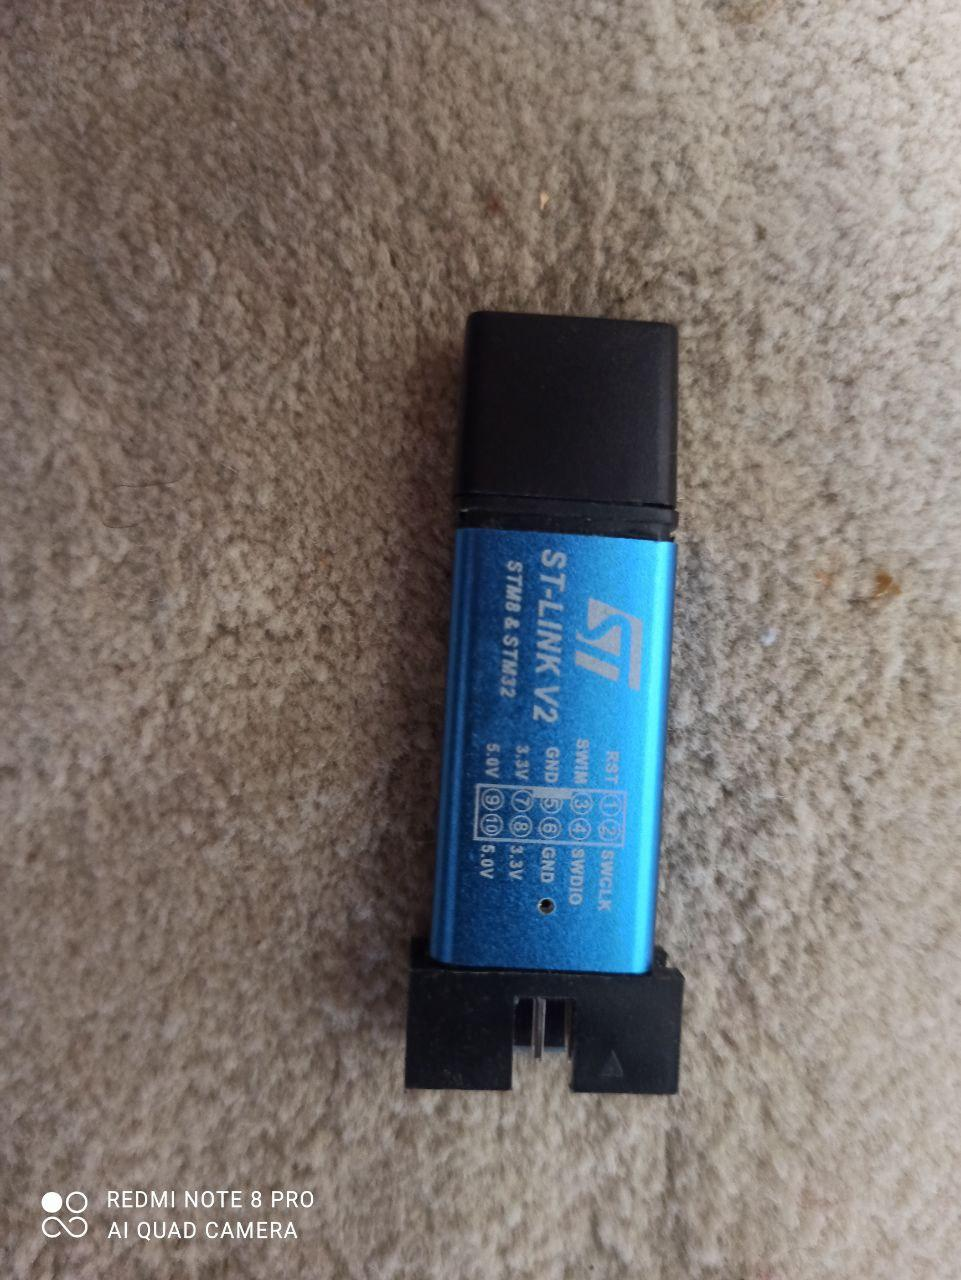
\includegraphics[width=\linewidth]{Assets/stlink.jpg}
		\caption{پروگرمر \متن‌لاتین{STLINK}}
		\label{fig:stlink}
	\end{subfigure}
	\begin{subfigure}[b]{0.5\textwidth}
		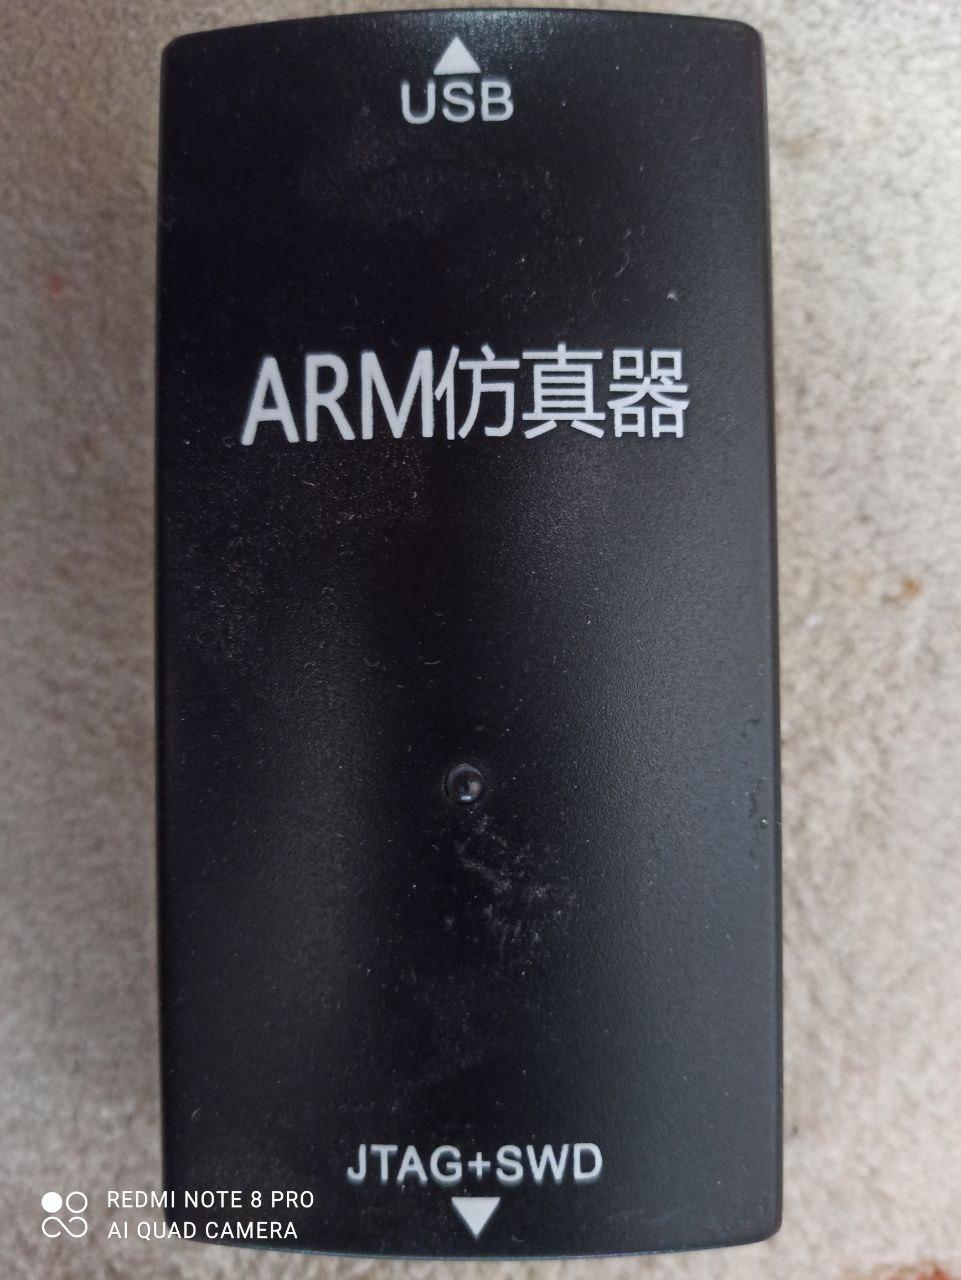
\includegraphics[width=\linewidth]{Assets/jlink.jpg}
		\caption{پروگرمر \متن‌لاتین{JLINK}}
		\label{fig:jlink}
	\end{subfigure}
	\caption{تصاویر پروگرمر‌های استفاده شده در این پروژه.}
	\label{fig:programmers}
\end{figure}

\قسمت{میکروکنترلر}

هسته اصلی پردازش در هر دو سمت ایستگاه و سنسور میکروکنترلر \متن‌لاتین{STM32f103CBT6} انتخاب شده است که با توجه به موجود بودن در بازار ایران و دارا بودن 2 عدد \متن‌لاتین{I\بالانویس‌متنی{2}C}\پانویس{Inter-Integrated Circuit}، 2 عدد \متن‌لاتین{SPI}\پانویس{Serial Peripheral Interface}، اینترفیس\پانویس{Interface} \متن‌لاتین{USB}\پانویس{Universal Serial Bus} و 3 عدد تایمر 16 بیتی نیاز به حداقل 1 عدد \متن‌لاتین{I\بالانویس‌متنی{2}C} (در سمت سنسور)، 1 عدد \متن‌لاتین{SPI} (در هر دو سمت)، اینترفیس \متن‌لاتین{USB} (در سمت ایستگاه)  و 1 عدد تایمر (در سمت سنسور) را برآورده می‌کند. همچنین حالت \متن‌لاتین{Sleep} و واحد \متن‌لاتین{RTC} موجود در این میکروکنترلرها به کاهش مصرف انرژی در وقفه‌های سه ساعته کمک می‌کند؛ به‌طوری‌که استفاده از سیستم باتری و پنل خورشیدی را ممکن می‌سازد.
